\chapter{Some plain text}

\blindtext

\chapter{A graphic with caption}

ü \Fref{fig:oats}! ä \Fref{fig:oats:a}! Look at that~\cite{newman2003structure}.

\begin{figure}
     \centering
     \subfloat[][a]{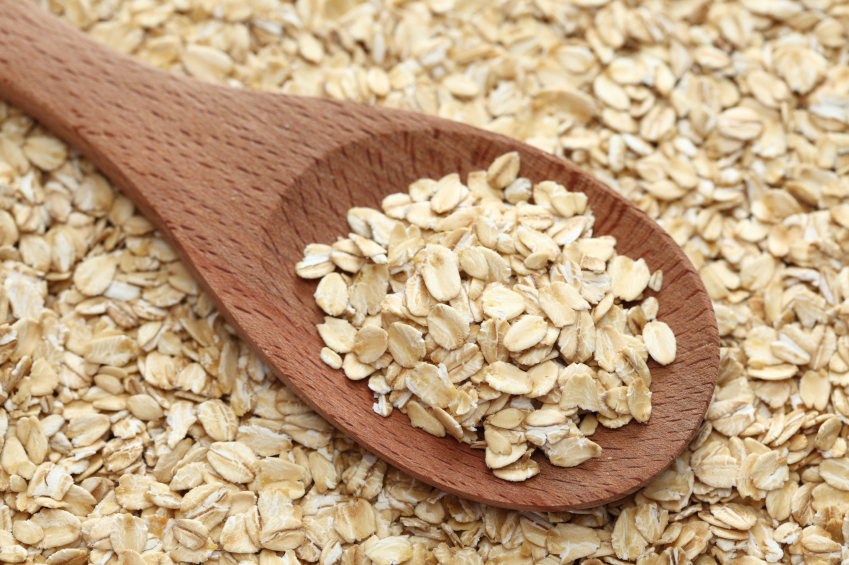
\includegraphics{oats.jpg}\label{fig:oats:a}}
     \subfloat[][b]{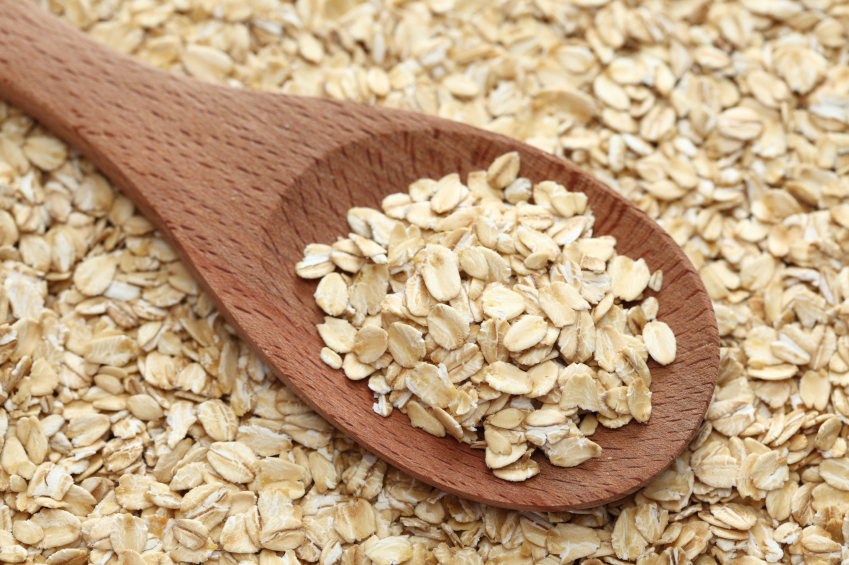
\includegraphics{oats.jpg}\label{fig:oats:b}}
     \caption[short toc caption]{Comparison of steady state results (a) x method (b) y method}
     \label{fig:oats}
\end{figure}


\begin{figure}
     \centering
     \subfloat[][a]{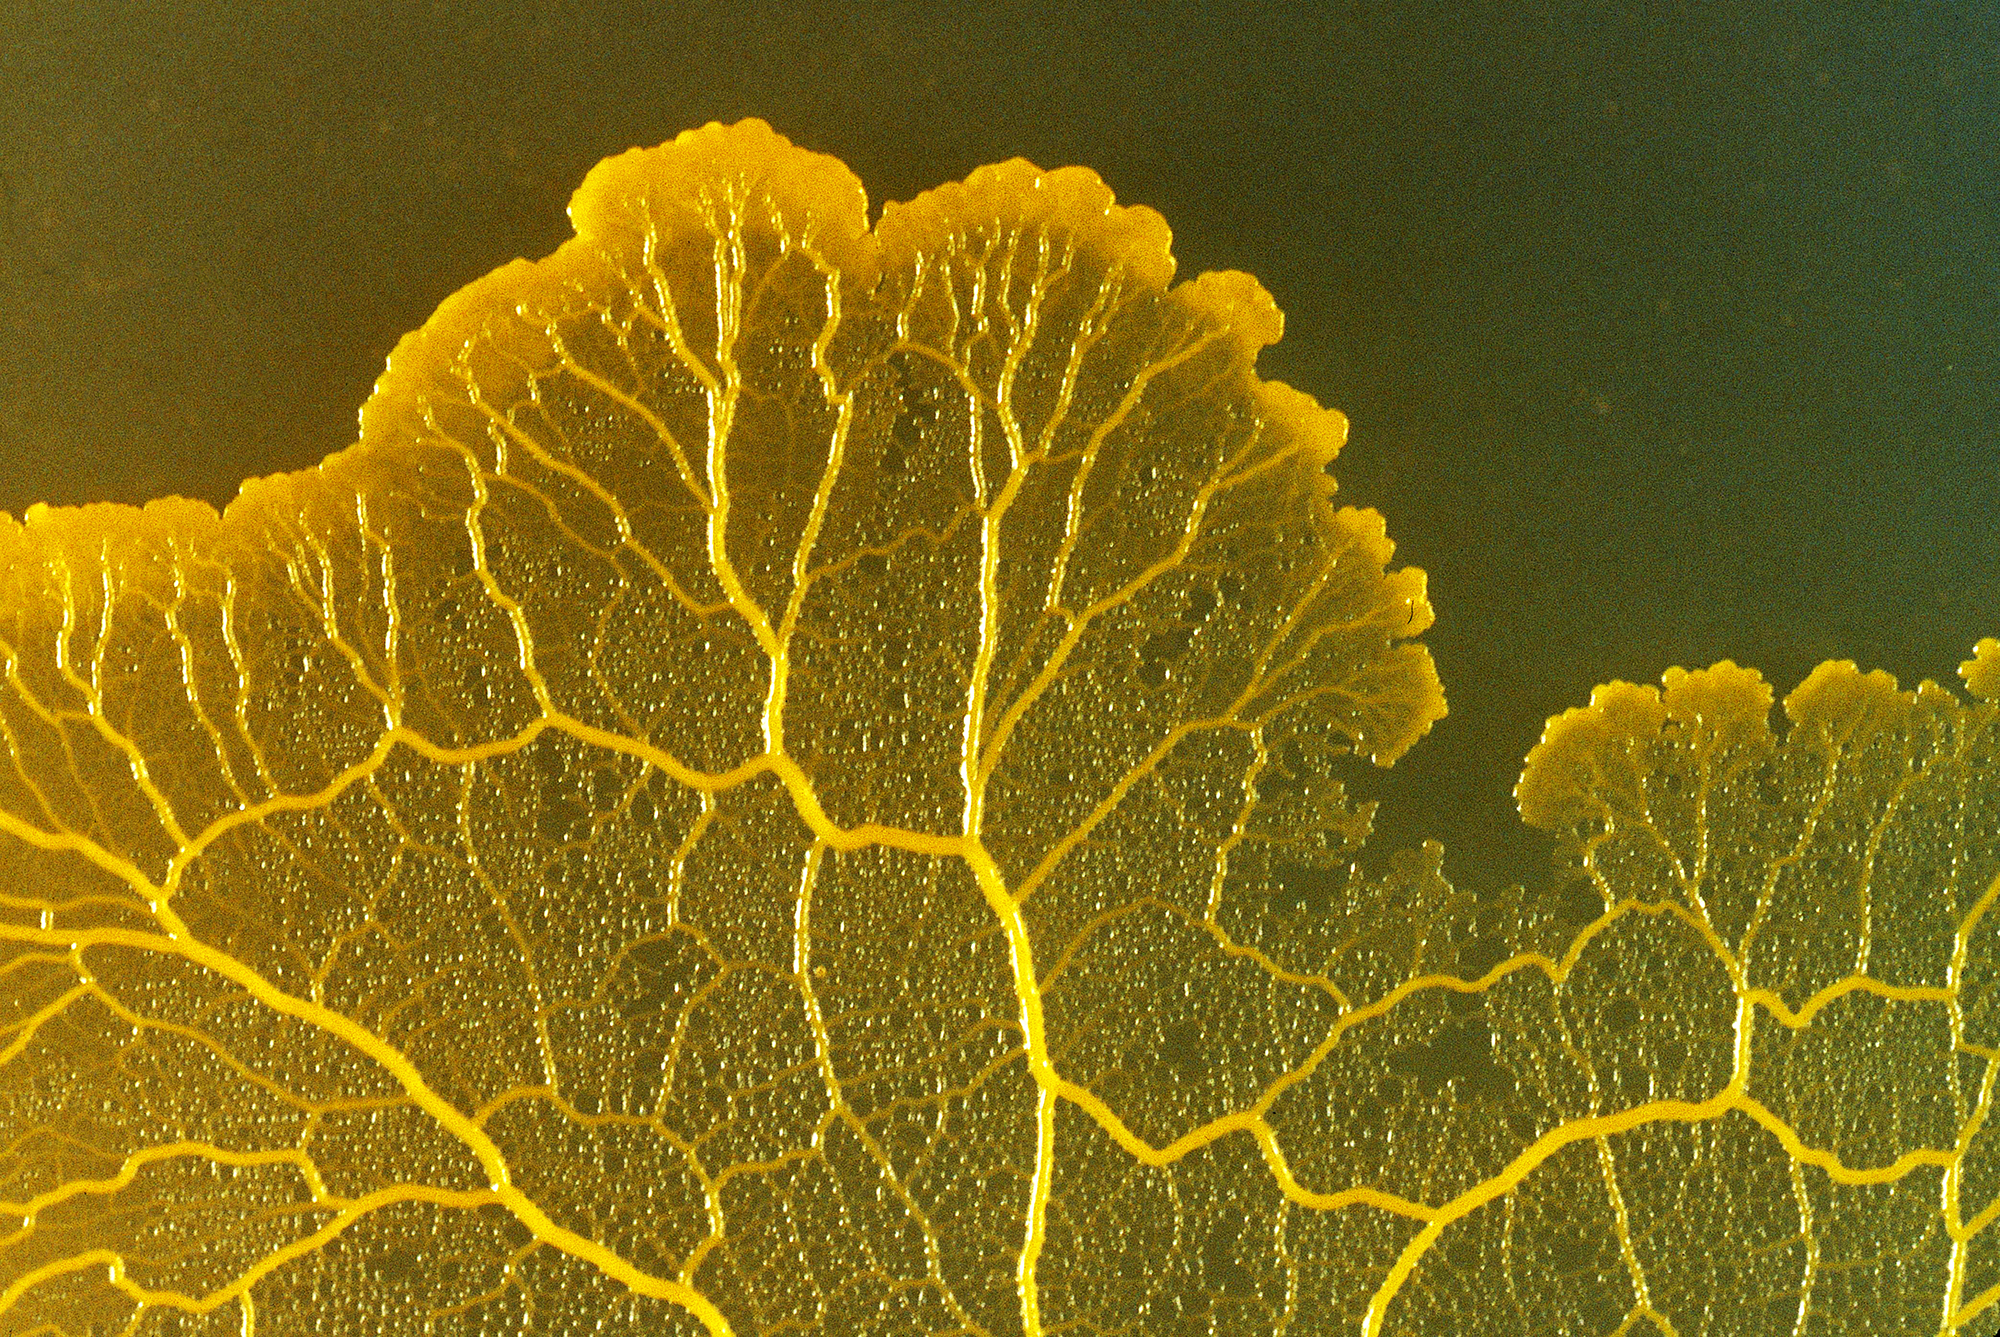
\includegraphics[width=0.5\linewidth]{slime.jpg}\label{fig:slime:a}}
     \subfloat[][b]{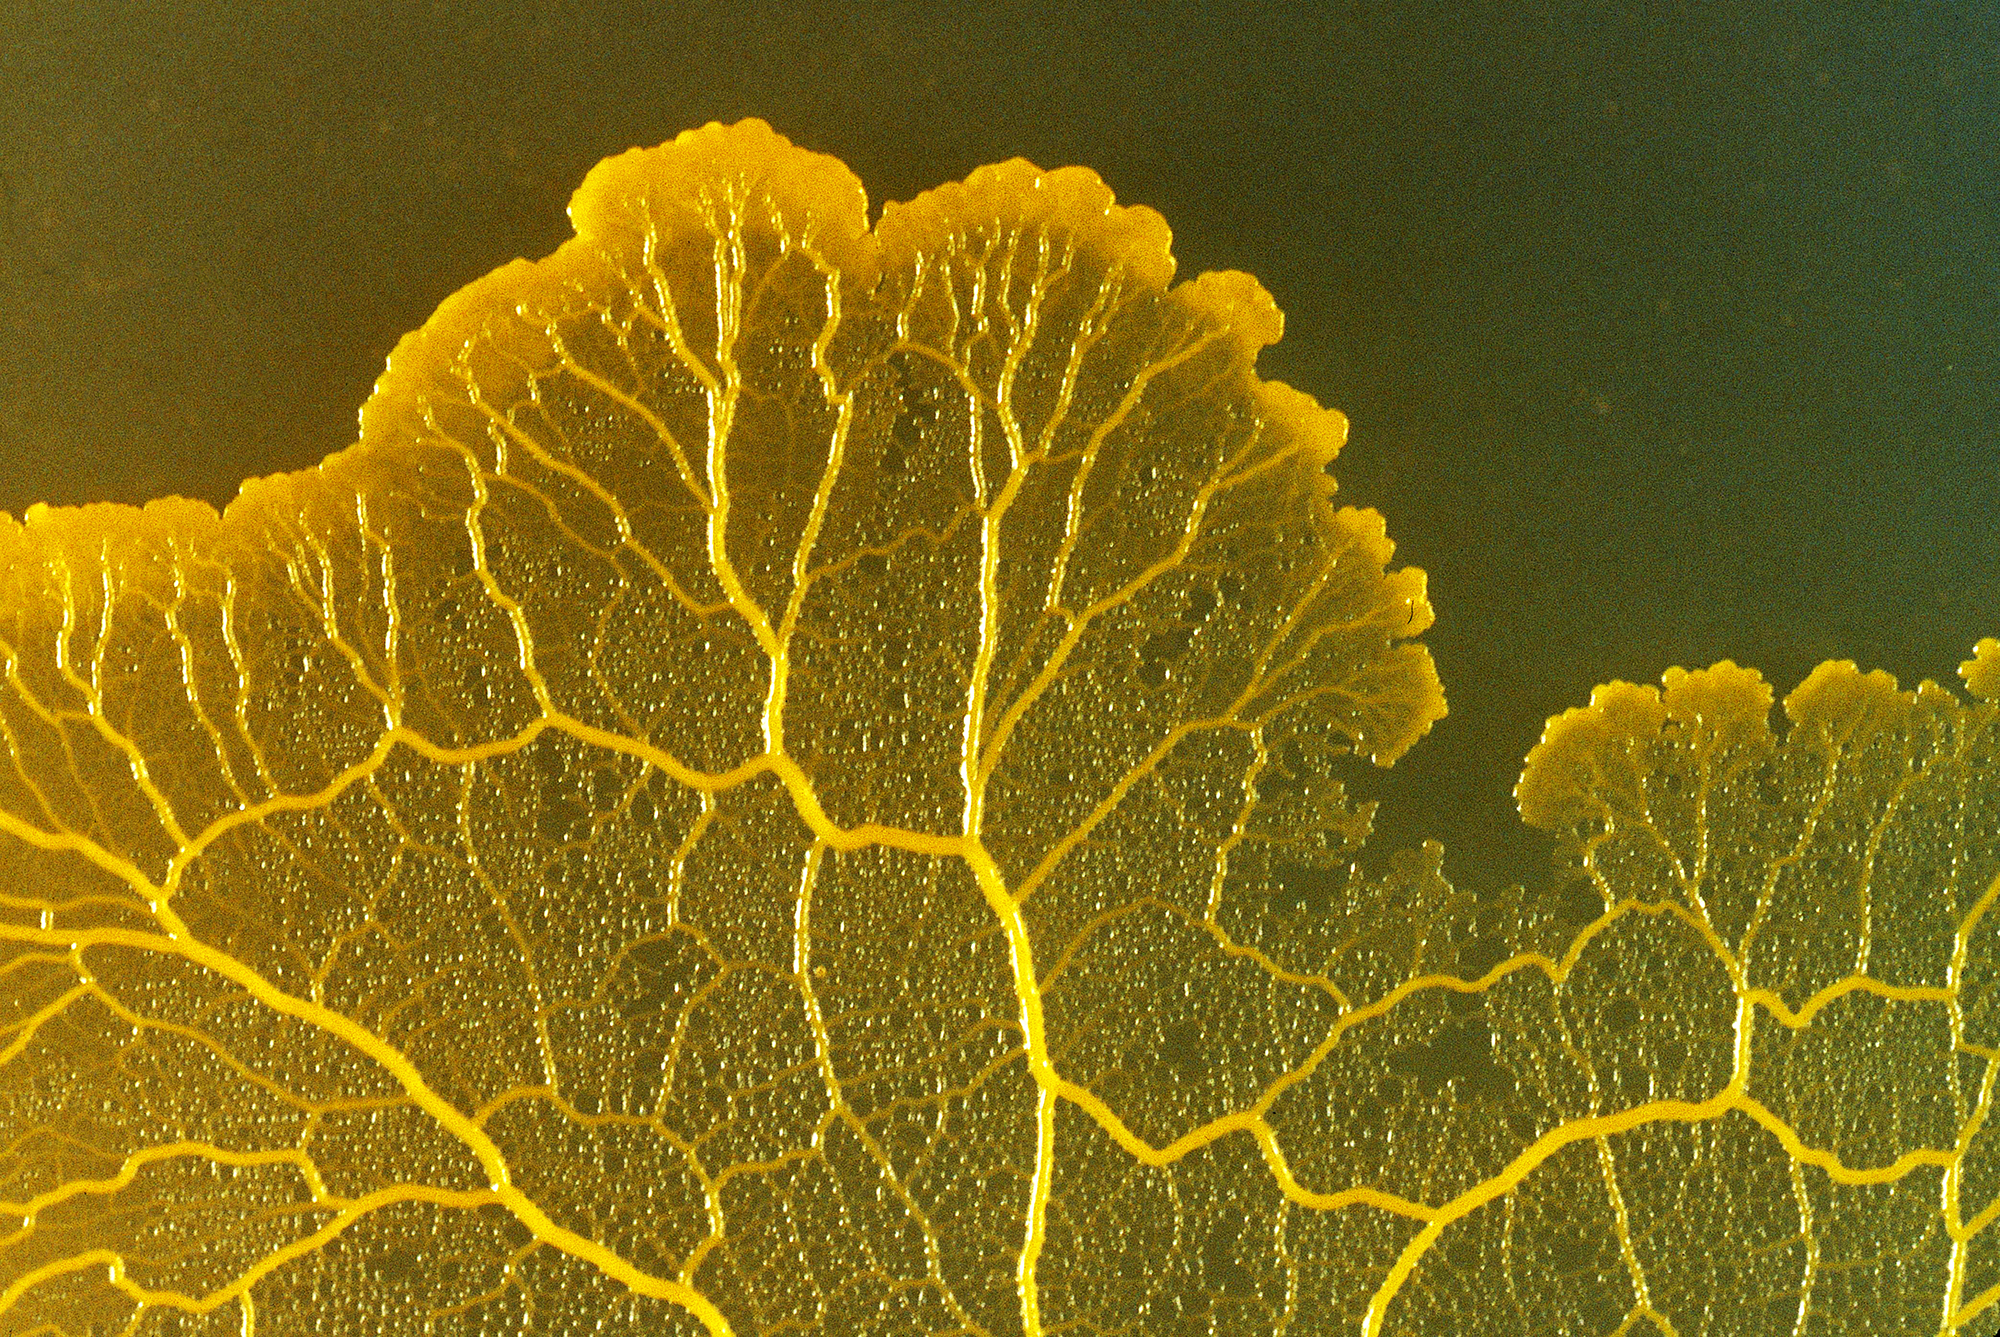
\includegraphics[width=0.5\linewidth]{slime.jpg}\label{fig:slime:b}}
     \caption[another short toc caption]{Hello there beautiful. \P is awesome.}
     \label{fig:slime}
\end{figure}

\chapter{A simple table with caption}

Hello, some citation here \Fref{tab:income}.

\begin{table}
	\centering
	\begin{tabular}{@{} l *4c @{}}
	\toprule
	 \multicolumn{1}{c}{Models}    & A  & B  & C  & D  \\ 
	\midrule
	 Model $X$ & X1 & X2 & X3 & X4 \\ 
	 Model $Y$ & Y1 & Y2 & Y3 & Y4 \\
	\bottomrule
	\end{tabular}
	\caption[another short toc caption]{Slime of type (a) and (b).}
	\label{tab:income}
\end{table}
